29. \begin{figure}[ht!]
\center{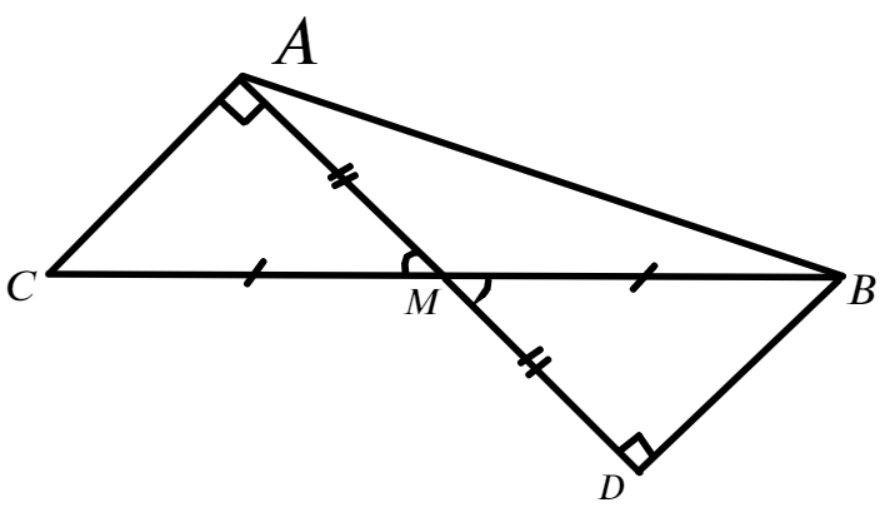
\includegraphics[scale=0.35]{g29.png}}
\end{figure}\\
Сделаем стандартное дополнительное построение: продлим медиану $AM$ на свою длину: $AM=MD.$ Тогда $\left.\begin{array}{l}AM=MD\text{ по построению},\\
 CM=MB\text{ ($AM$ --- медиана)},\\ \angle BMD=\angle CMA\text{ (вертикальные).}\end{array}\right\}\Rightarrow
\Delta BMD=\Delta CMA\text{ по I признаку}\Rightarrow AC=BD$ и $\angle BDM=\angle CAM=90^\circ.$ Треугольник $BAD$ является прямоугольным и в нём $AB=2AC=2BD,$ значит катет $BD$ лежит напротив угла в $30^\circ,$ поэтому $\angle BAM=30^\circ.$ Таким образом, $\angle BAC=90^\circ+30^\circ=120^\circ.$\\
